

\begin{flushleft}

	
{\color{Blue}{\subsection{Overview}}}
Both Data4Help ad AutomatedSOS are complex services due to the large set of technologies involved in their functionalities. To have a full comprehension of the overall architecture, it is necessary to abstract the entire system, starting the analysis from the customer perspective. Here, in fact, the main challenge is related to device management and data representation, since a large variety of sensors (supported by the service), can be connected and send data simultaneously. Each health indicator sample provided to the app should be processed at first in order to match a common data structure, then sent to the server. Since a D4H user is automatically an ASOS user at the first run of the relative application, it may happen that the same will use both the applications in tandem. This leads to a problem of data redundancy, since the server could receive two samples from the same monitoring device. The problem should easily solved by the server, if it was not computational expensive for growing workloads. This part of the business logic could be easily managed by the apps through a mechanism of message exchanging to synchronize the sensor accesses and preventing the .   To this purpose, from an high-level perspective it is useful to rely on the following picture:

\begin{figure}[H]
	\centering
	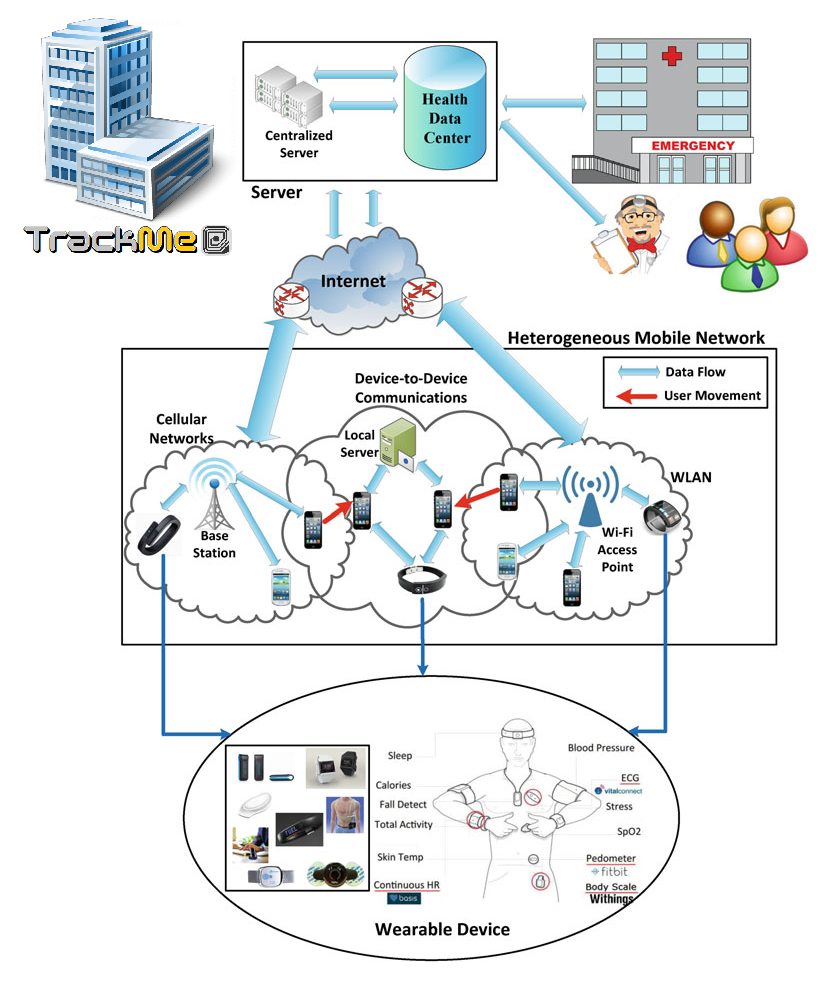
\includegraphics[scale=0.7]{images/system_perspective}
	\caption{}
\end{figure}


 


{\color{Blue}{\subsection{Component View}}}
T
{\color{Blue}{\subsubsection{Client Side}}}
Starting from the interface to the external sensors, the main problem related to the app separation is due to the fact that if the applications are running at a certain moment both of them could theoretically access the same monitoring device, providing to the server an identical sample. As anticipated in the Overview part, both the applications at clien side implement a personal hardware interface to the connected monitoring devices. This decision seems to introduce redundancy in code since a simple third service running in background could manage the connected devices and dispatch data between the two applications, unfortunately communication among running processes follows strict rules in many mobile OSs, someone only allows message exchanging. This makes more difficult to implement a mechanism of access to the monitoring sensors involving at most three different processes. Furthermore, relying on an HW manager service exposes both the apps to possible internal DOS attacks, since another malicious app could flood of messages the background service preventing the main application to allocate accesses to connected sensors.

\begin{figure}[H]
	\centering
	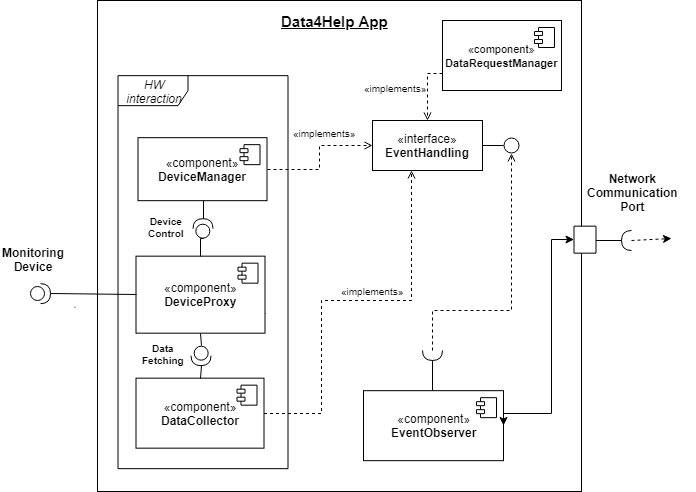
\includegraphics[scale=0.6]{images/uml/D4H_client_component}
	\caption{}
\end{figure}

It has been decided to create a communication interface between D4H and ASOS, for synchronizing data collection and preventing both the applications to access the same information. This task should be protected in order to avoid other processes to send false messages to one of them. A security toolkit provides encryption mechanism to this end.
\begin{figure}[H]
	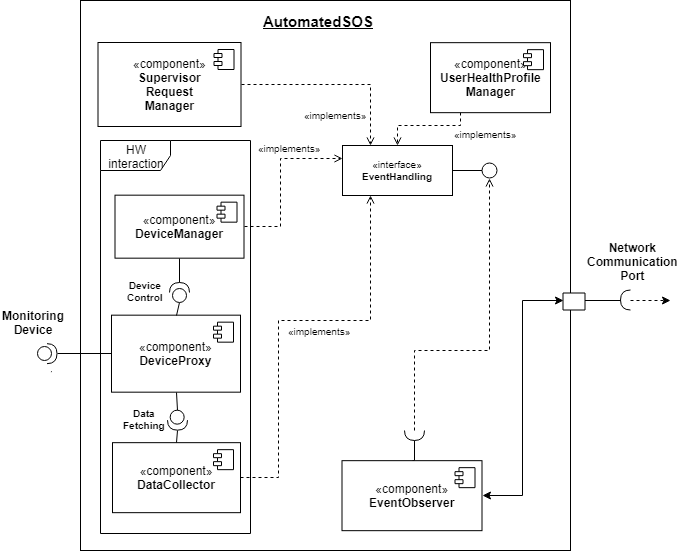
\includegraphics[scale=0.6]{images/uml/ASOS_client_component}
	\caption{}
\end{figure}


\begin{figure}[H]
	\centering
	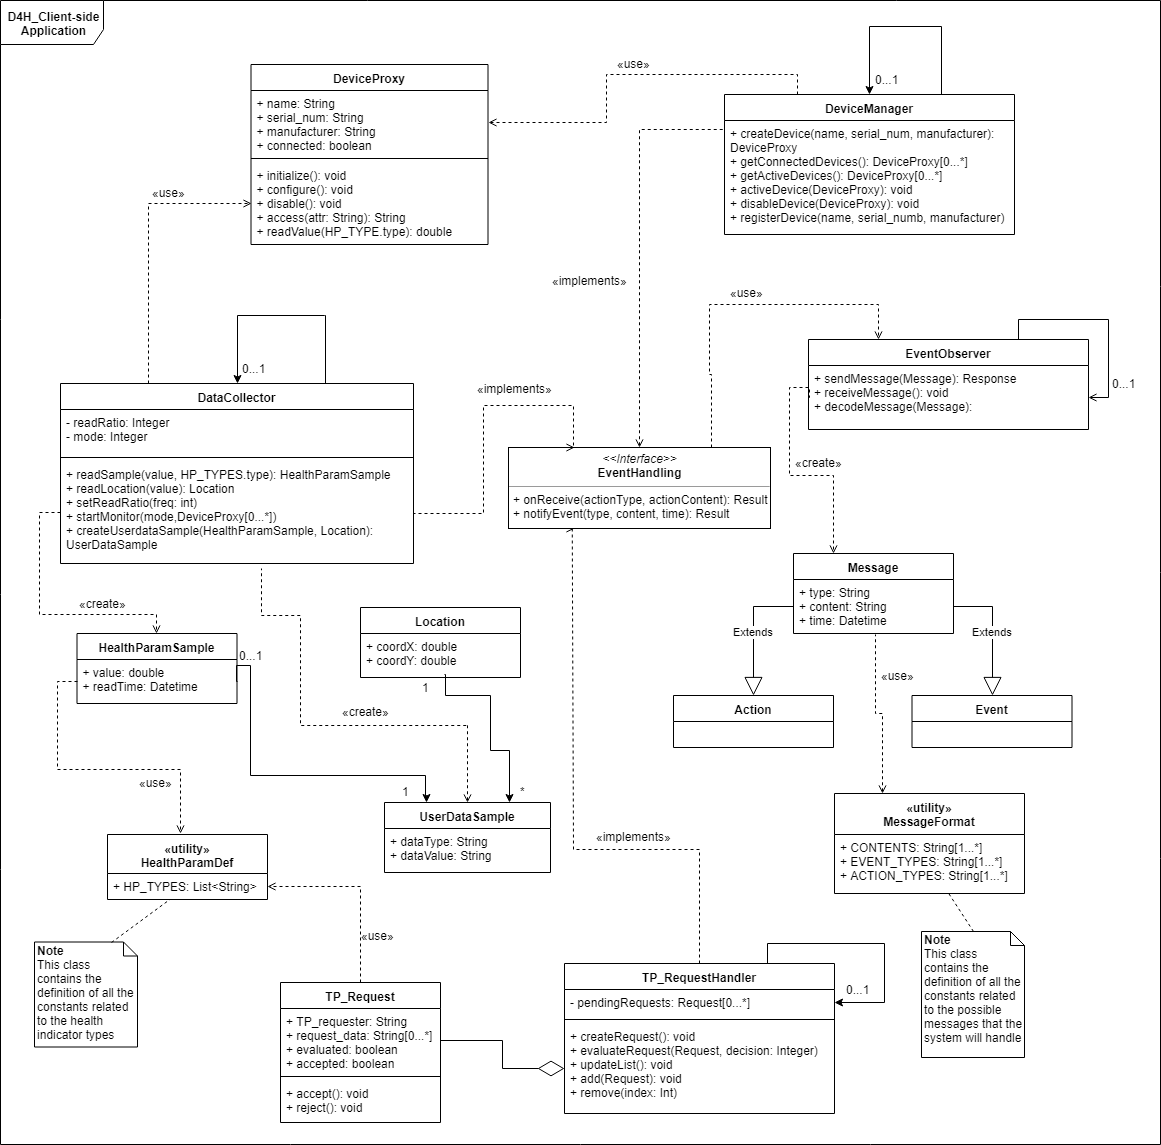
\includegraphics[scale=0.33]{images/uml/D4H_client_class}
	\caption{}
\end{figure}


\begin{figure}[H]
	\centering
	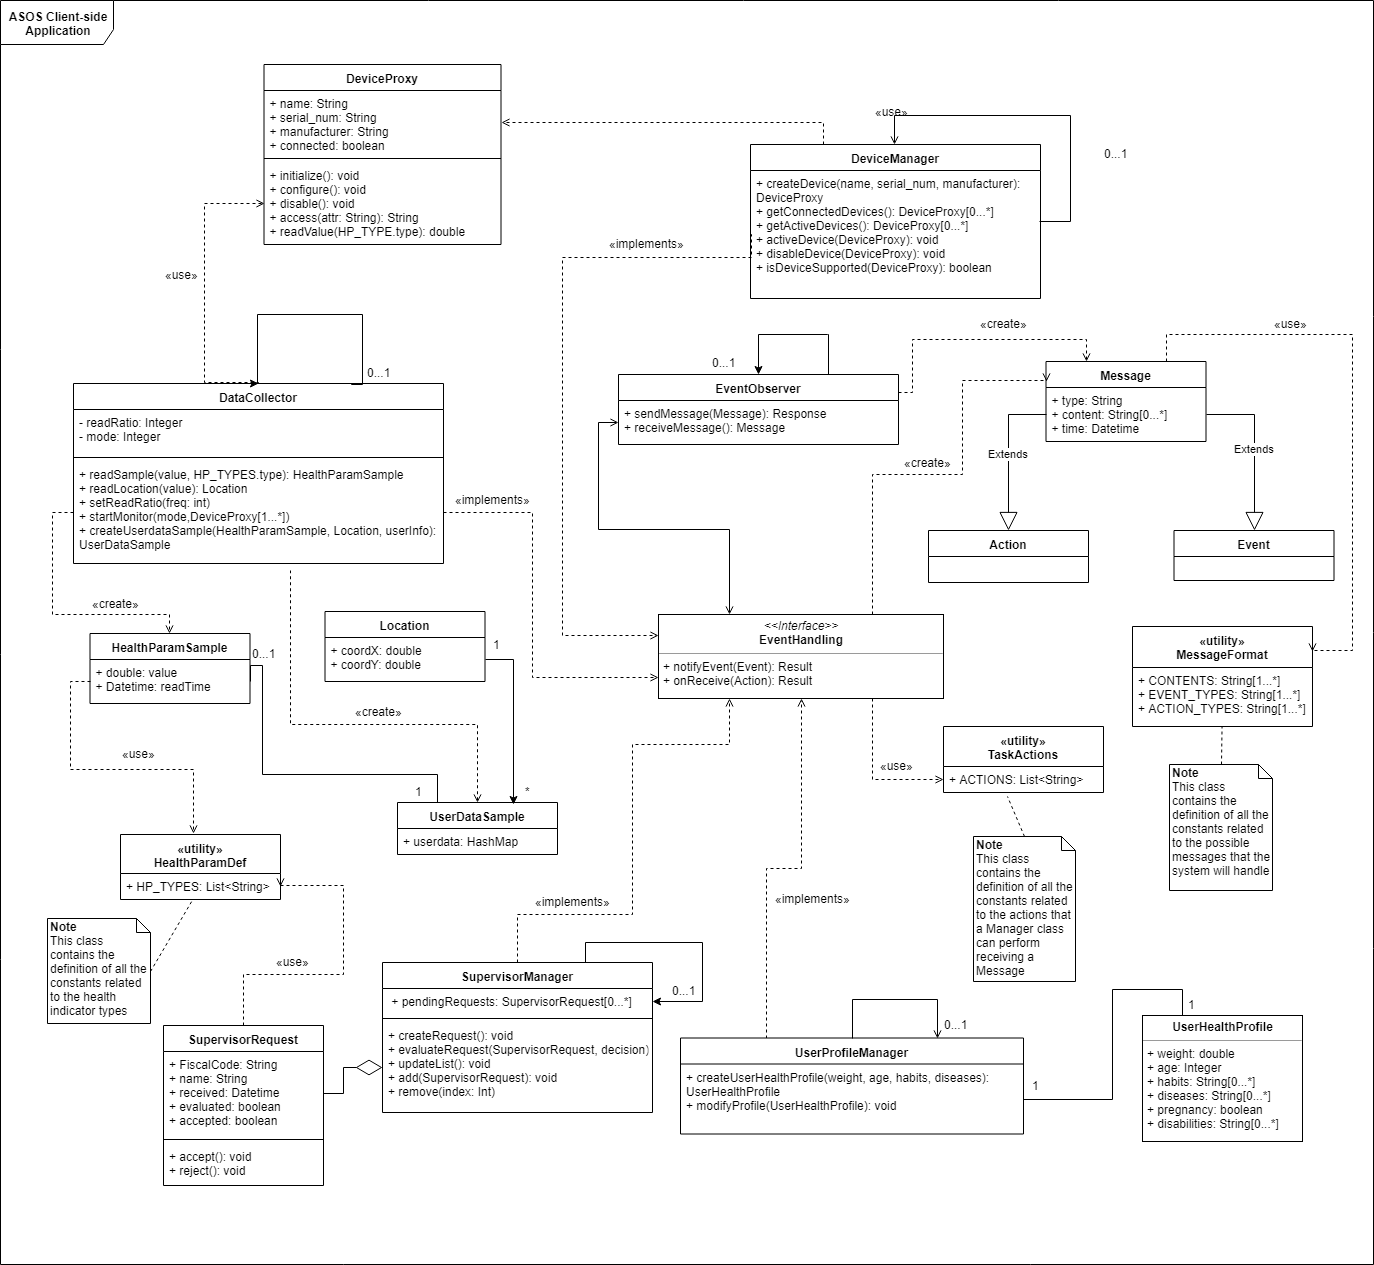
\includegraphics[scale=0.33]{images/uml/ASOS_client_class}
	\caption{}
\end{figure}

\begin{figure}[H]
	\centering
	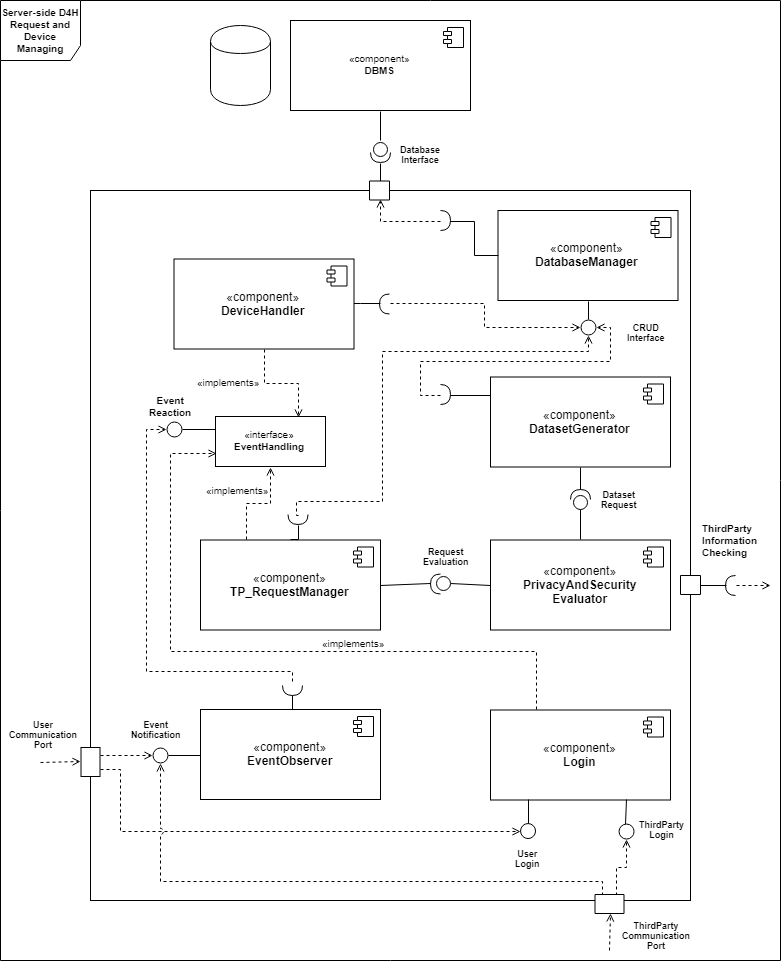
\includegraphics[scale=0.5]{images/uml/D4H_server_requestManaging_component}
	\caption{}
\end{figure}


\begin{figure}[H]
	\centering
	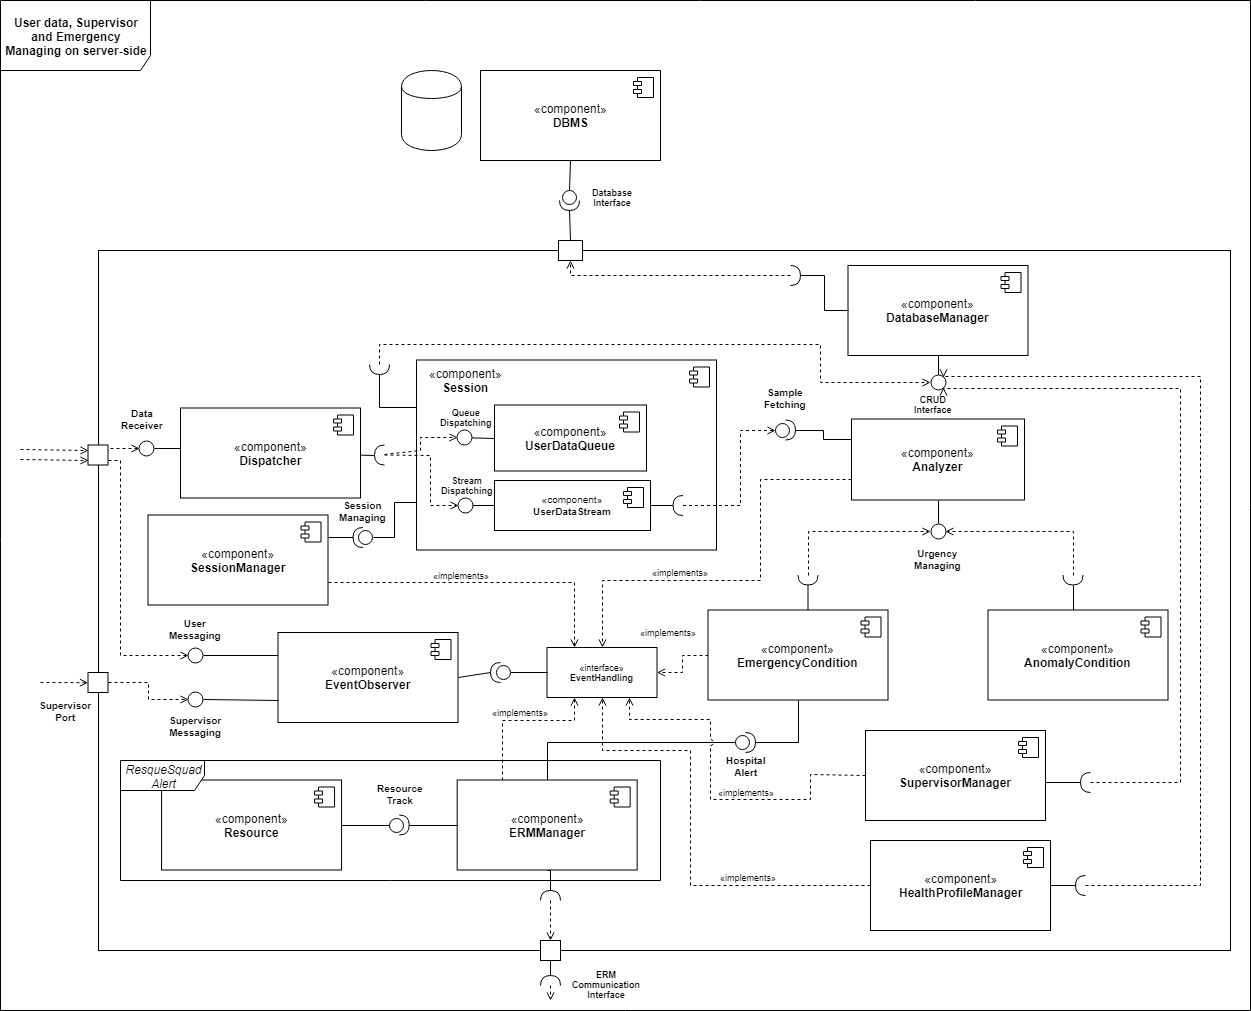
\includegraphics[scale=0.4]{images/uml/ASOS_server_emergency_component}
	\caption{}
\end{figure}

{\color{Blue}{\subsection{Deployment View}}}


{\color{Blue}{\subsection{Runtime View}}}


{\color{Blue}{\subsection{Component Interfaces}}}


{\color{Blue}{\subsection{Selected Architectural Styles and Patterns}}}


{\color{Blue}{\subsection{Other Design Decisions}}}
	

\end{flushleft}
